\chapter{Common Language Infrastructure}
\label{chap:cli} 
The \idx{Common Language Infrastructure} (\idx{CLI}), not to be confused with \idx{Command Line Interface} with the same acronym, is a technical standard developed by Microsoft \cite{iso23271:2012, ecma335}. The standard specifies a language, its format, and a run-time environment that can execute the code. The main feature is that it provides a common interface between many languages and many platforms, such that programs can collaborate in a language agnostic manner and can be executed on different platforms without having to be recompiled. Main features of the standard are:
\begin{description}
\item[Common Type System (CTS)]\idxs{Common Type System}\idxs{CTS} which defines a common set of types that can be used across different languages as if it were their own.
\item[Metadata]\idxs{Metadata} which defines a common method for referencing programming structures such as values and functions in a language independent manner.
\item[Common Intermediate Language (CIL)]\idxs{Common Intermediate Language}\idxs{CIL} which is a platform-independent, stack-based, object-oriented assembly language that can be executed by the Virtual Execution System.
\item[Virtual Execution System (VES)]\idxs{Virtual Execution System}\idxs{VES} which is a platform dependent, virtual machine, which combines the above into code that can be executed at runtime. Microsoft's implementation of VES is called \idx{Common Language Runtime} (\idx{CLR}) and uses \idx{just-in-time} compilation.
\end{description}
The process of running an F\# program is shown in Figure~\ref{fig:cliOverview}\jon{update figure}: First the F\# code is compiled or interpreted to CIL. This code possibly combined with other CIL code is then converted to a machine readable code, and the result is then executed on the platform.
\begin{figure}
  \centering
  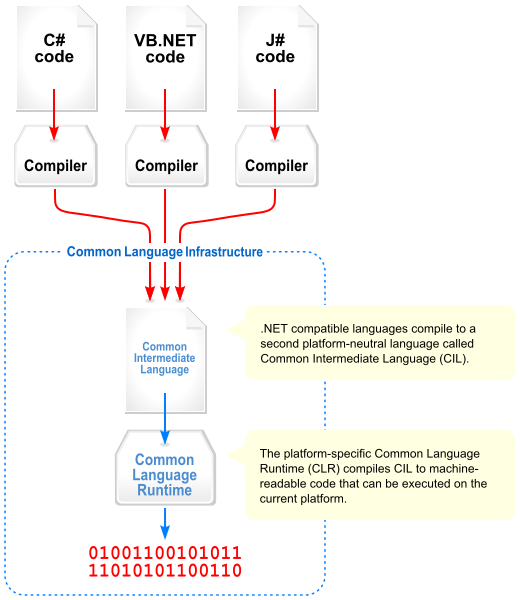
\includegraphics[width=0.45\textwidth]{Overview_of_the_Common_Language_Infrastructure}
  \caption{Visual overview of CLI. Figure by Jarkko Piiroinen - Own work, Public Domain, \url{https://commons.wikimedia.org/w/index.php?curid=3602584}.}
  \label{fig:cliOverview}
\end{figure}

CLI defines a \idx{module} as a single file containing executable code by VES. Hence, CLI's notion of module is somewhat related to F\#'s notion of module, but the two should not be confused. A collection of modules, a \idx{manifest}, and possibly other resources, which jointly define a complete program is called an \idx{assembly}. The manifest is the description of, which files are included in the assembly together with its version, name, security information, and other bookkeeping information.

%%% Local Variables:
%%% TeX-master: "fsharpNotes"
%%% End:
